\documentclass[conference]{IEEEtran}

\usepackage{url}

\hyphenation{op-tical net-works semi-conduc-tor}

\usepackage[czech]{babel}
\usepackage[utf8]{inputenc}   % pro unicode UTF-8
\usepackage{gensymb}

\usepackage[pdftex]{graphicx}
\graphicspath{{./images/}}
\DeclareGraphicsExtensions{.pdf}

\renewcommand\IEEEkeywordsname{Keywords}

\addto{\captionsczech}{
	\renewcommand{\abstractname}{Abstract}
	\renewcommand{\refname}{References / Reference}
}

\begin{document}

\title{Zálohování počítačových dat na papír\\ a jejich rekonstrukce pomocí neuronové sítě}

\author{
	\IEEEauthorblockN{Bc. Miroslav Pokorný}
	\IEEEauthorblockA{Faculty of Informatics and Management\\
		University of Hradec Králové,\\
		Hradec Králové, Czech Republic\\
		miroslav.pokorny@uhk.cz}
}

\maketitle

\begin{abstract}

V dnešní době produkujeme velké množství dat. Některá tato data jsou, ale důležitější/citlivější povahy než jiná a mají pro nás jako uživatele daleko větší cenu. Proto je zapotřebí tato data nějakým způsobem efektivně a trvale zálohovat, abychom o ně nepřišly, nebo alespoň minimalizovali pravděpodobnost jejich ztráty. V této práci řešíme možnost zálohy počítačových dat na papír za pomoci omezené sady textových znaků (písmen) a jejich zpětnou rekonstrukci pomocí konvoluční neuronové sítě, kterou v rámci této práce učíme (trénujeme). Na omezené testovací sadě se podařilo dosáhnout 100\% úspěšnosti klasifikace jednotlivých znaků (písmen). Ačkoli výstupem této práce není produkční řešení, tak se ukazuje, že po dalším výzkumu a implementaci by se mohlo jednat o zajímavé řešení v problematice zálohování dat na papír.

\end{abstract}

\vspace{5mm}

\begin{IEEEkeywords}
	Záloha dat, neuronová síť, base32, base64, strojové učení, počítačová data na papíře
\end{IEEEkeywords}

\IEEEpeerreviewmaketitle

\section{Introduction / Úvod}

Žijeme v digitální době, a již s těží bychom našli nějakou činnost, kterou bychom nebyly schopni pomocí počítače nebo nějakého chytrého zařízení (chytrý telefon, tablet,...) udělat, nebo si ji minimálně ulehčit \cite{Ubicomp2001}.  Na internetu se registrujeme do stále nových služeb, a v mnohých případech za ty to služby i platíme nemalé peníze. Čím více máme těchto účtů tím více bychom měli mít i hesel, aby v případě narušení bezpečnosti nebo důvěry v nějaké z nich neměly za následek i kompromitaci ostatních. Velké množství hesel je tak zapotřebí nějak rozumně spravovat, z tohoto důvodu již vznikli chytré prográmky pro správu hesel, jako je například KeePass,... Produktem takovéhoto programu je pak, ale binární soubor, který je potřeba nějak chránit proti ztrátě, protože obsahuje velké množství důležitých dat. Kam rozumně, ale takový důležitý soubor za zálohovat? Pokud jej budeme mít je na jednom počítači, můžeme o něj snadno přijít. Záloha na další fyzické zařízení (například flash disk) také není 100\% trvalé a vhodné zálohovací zařízení \cite{DataStorageLifespans}. Nahrávání takovéhoto souboru do cloudových úložišť je také potencionálně nebezpečné, a vyžaduje velkou důvěru vůči poskytovateli tohoto řešení \cite{ALSMADI2018218}\cite{7MostFamousCloudSecurityBreaches}\cite{HowSecureIsYourData}. 

Abychom mohli data zapsat na papírové médium je zapotřebí počítačová data nějakým vhodným způsobem zakódovat, tak abychom je byly i schopni snadno rozkódovat. Můžeme zvolit různé metody zakódování dat od grafického, pro člověka ne příliš hezky čitelného, až po textového, který je člověk v případě potřeby schopen alespoň částečně interpretovat. Jako vhodné řešení vyplývá použít metodu, která v případě, že selže program určený k rekonstrukci dat, umožní data do počítače zadat i samotnému uživateli (jedná se o krajní případ, ke kterému by nemělo docházet). 

Zvolíme-li tedy, že data budeme kódovat do textové podoby, tak aby byla ,,čitelná člověkem`` (například kódování binární dat do textové podoby pomocí kódování Base64, Base32,... \cite{RFC4648}), tak musíme také najít vhodný způsob jakým data budeme načítat zpátky do počítače. Jelikož máme data na papíře je nutné tyto obrazová/textová data přenést zpět do počítače za pomoci nějakého skenovacího zařízení, jehož výstupem je rastrový obrázek. Jakmile máme obrazová data naskenována v počítači můžeme začít s ,,automatizovanou`` rekonstrukcí těchto dat. Klasické OCR (optical character recognization) algoritmy nejsou pro tyto účely příliš vhodné \cite{RecognizationVehicleLicencePlates}, protože fungují spolehlivě hlavně pokud v textu, který dekódují existuje nějaký kontext (tj. data mají význam slov) a algoritmus je schopen v případě nejistoty rozhodnout, na základě ostatních znaků, nebo slov, který znak je v daném místě pravděpodobnější. V případě dekódování zálohovaných dat je ale nutné dosáhnout veliké spolehlivosti dekódování dat, protože i relativně vysoká spolehlivost 99\% by znamenala, že se data nemusí podařit správně dekódovat.

Jelikož máme data v obrazové podobě a nemůžeme uplatnit algoritmy OCR, je zapotřebí aplikovat jiné řešení. Jako jedno z možných řešení je využití klasifikace jednotlivých písmen textu pomocí konvuločních neuronových sítí \cite{NIPS2010_4136}\cite{doi:10.1080/2150704X.2018.1526424}\cite{SEO2019328}. Spolehlivost takovéhoto řešení bude závislá na kvalitě naučení neuronové sítě a přípravě/zpracováním vstupních dat před vstupem do klasifikačního procesu neuronové sítě.

Při dekódování dat je nutné také mít informaci o tom, zda se podařilo data do dekódovat správně, nebo zda během klasifikace došlo k chybě a nějaké znaky (písmena a čísla) jsou dekódovány nesprávně a je nutné provést nějaké korekční kroky. K ověření integrity dat je vhodné použít nějakou metodu kontrolního součtu. Pro tento účel lze využít hashovacích funkcí, které spočítají hash (otisk) dat (například hashovací funkce MD5, SHA1,... \cite{RFC3174}). V případě, že se data budou lišit, tak tyto otisky budou navzájem různé (je nutné volit správnou metodu spočtení tohoto otisku, tak aby možnost kolize byla nepravděpodobná). Pokud po rekonstrukci dat, a následném spočtení kontrolního součtu bude kontrolní součet odpovídat, můžeme s téměř naprostou jistotu prohlásit, že data jsou dekódována správně. Kontrolní součet je zapotřebí vhodně uložit, tak aby byl pro počítač snadno a správně dekódovatelný. V dnešní době umějí počítače a chytré telefony snadno dekódovat data uložená do QR kódu (za předpokladu, že ukládáme relativně malé množství dat).

\section{Problem definition / Definice problémů}

Pokud budeme chtít zálohovat počítačová data na papír, tak se nám otevírá daleko více možností, než by se na první pohled mohlo zdát. V minulosti počítače běžně používaly papír jako paměťové médium \cite{PaperDataStorage}. Na tzv. děrné štítky se ukládaly jak data, tak programy, které počítače zpracovávaly. Děrný štítek jako takový neměl nikdy příliš velkou kapacitu. Děrný štítek 5081 (5081 punch card) mohl nést informaci až o 80 alfanumerických znaků. Ačkoliv děrné štítky byly spolehlivé, v dnešní době se jedná o zastaralou technologii a pro jejich vytvoření/čtení je zapotřebí specializovaný hardware, který v dnešní době již není běžný. 

Další možnosti jak zálohovat data na papír je využití nějakého prostředku pro automatizovaný sběr dat. Příkladem těchto prostředků mohou být kódy typu data matrix, QR kód, nebo EAN čárový kód. Tyto kódy jsou standardizované a existuje velké množství softwarových řešení, které umí tyto kódy generovat a číst. Nevýhodou těchto kódů pak je, že jsou pro člověka velice těžce čitelné, a jejich rozluštění v případě potřeby by pro člověka mohlo být velice náročné (ne-li nemožné).

Jedno možné řešení implementoval Grant Trebbin \cite{GrantTrebbin}. Jeho řešení neimplementuje žádný samostatný program, ale pouze využívá nástrojů/utilitek dostupných na linuxových operačních systémech. Jeho řešení spočívá v tom, že data nejprve zakóduje do kódování base64. Poté data rozseká na menší části, tak aby se vešli do QR kódu. Poté pro každý úsek dat vygeneruje jeden QR kód. Následně jsou vytvořeny jednotlivé stránky, které obsahují více QR kódu, tyto stránky pak mohou být vytištěny. Po načtení kódu zpět do počítače, jsou kódy postupně dekódovány a z jednotlivých částí je slepen původní base64 soubor. Jakmile existuje soubor s base64 textem, může se opět dekódovat do původní binární podoby. Toto řešení má výhodu ve využití běžně dostupných nástrojů v operačním systému. Nevýhodu je absence automatice řešení, tj. pro kódování a dekódování dat je nutné, aby uživatel spouštěl příkazy ručně.

Alternativní možností jak zálohovat data na papír (v tomto případě se nemusí jednat jen o papír, ale jakékoliv vizuální médium) je tzv. dataglyph \cite{DataGlyphsFreePatenstsOnline}\cite{dataglyphs}. V tomto případě jsou binární data zakódována do vizuální podoby pomocí sekvencí šikmých čar (lomítek a zpětných lomítek), které reprezentují jedničky a nuly dat. Jedná se o jeden z typů ,,čárových kódů``, které jsou snadno zpracovatelné počítačem. Tento typ kódu lze kombinovat (zakódovat) dohromady s obrázkem, tak aby byl pro člověka na první pohled skrytý, ale pro počítač stále dobře čitelný. Toto řešení není příliš vhodné pro uložení velkého množství informací. Další nevýhodou tohoto řešení je to, že nemá otevřený zdrojový kód (open source) a v případě, že by jsme jej chtěly využít budeme potřebovat patřičnou licenci.

Dalším jednoduchým prográmkem, který zálohuje data na papír je \emph{paperbackup.py} \cite{PaperBackup}. Jak již název napovídá jedná se o řešení implementované v programovacím jazyce python. Paperbackup je primárně určen pro zálohy šifrovacích klíčů (GnuPG (v ASCII podobě), SSH) nebo šifrovaného textu. Výstupem programu je pdf soubor, který může být vytištěn na papír. Obsahem tohoto souboru jsou stránky obsahující QR kódy, u každého kódu je textová informace o jakou část dat se jedná. Na konci souboru je pak, pro případ selhání dekódování QR kódů, vytištěn plaintextový obsah zálohovaného souboru. 

Nejvíce propracovaným existujícím řešením, pro zálohu dat na papír se zdá být aplikace PaperBack \cite{PaperBak}. PaperBack je open source řešní, šířené pod licencí GNU General Public License, version 3. Tato aplikace ukládá data na papír ve formě bitmapových obrázků (jsou velice podobné QR kódům \cite{ScanningQrCodes}, nebo spíše data matrix kódům, protože neobsahují ,,finder pattern`` čtverce, tak jako QR kódy), které mají formát specificky vyvinutý pro účely této aplikace. Toto řešení umí v případě kvalitní tiskárny uložit až 500000 bajtů nekomprimovaných dat na jednu stranu A4. Řešení PaperBack má integrované komprimační algoritmy, pomocí kterých je v ideálním případě možné uložit na jednu stranu A4 až 3 MB dat. Další vlastností této aplikace je integrovaný mechanismus šifrování dat. Data předaná aplikaci, aby je zálohovala, mohou být před vytištěním zašifrována, pomocí algoritmu AES-192, tak aby v případě, krádeže papíru byla data ochráněna, tj. útočník sice získá papíry s daty, ale bez správného hesla, je nebude schopen obnovit.

Všechny uvedené existující aplikace/metody využívají společný princip, kdy data, které zálohujeme jsou uloženy na papír ve formě grafické reprezentace (tj. jedná se o nějakou bitmapu, ve které jsou data zakódována). Výhodou uložení dat do bitmapy (například QR kódu) je to, že jsme schopni uložit relativně velké množství informací na malou plochu papíru. Rekonstrukce těchto dat pak záleží na dvou faktorech. Prvním je kvalita tiskárny, pomocí které budou data na papír tištěna, tak aby se nějaká informace neztratila už během tisku. Druhý důležitý faktor je načítání dat zpět do počítače. Pro účely načtení dat je nutné mít nějaké kvalitní skenovací zařízení, tak aby se žádná informace neztratila při načítání dat do počítače. 

Nevýhodou těchto řešení je to, že pro obnovu dat je zapotřebí mít k dispozici původní program. V případě, že při dekódování program selže, nebude možné (nebo to bude nesmírně složité) data obnovit. Může také nastat situace, kdy dekódovací program nebude po nějaké době spustitelný na moderním stroji (například program mohl být napsán pro v době dekódování již nepodporovaný operační systém, atd...). Tento problém nemusí být tak významný v případě open source řešení (je možné provést port na modernější operační systém/platformu). V případě proprietárních řešení mohou data být ztracena.

Žádný z existujících řešení nevyužil možnosti data, zálohovat zakódovaná v textové podobě, tak aby v případě potřeby (selhání dekódovacího programu) bylo možné, aby je dekódoval sám člověk. Z tohoto důvodu budeme v této práci dále pojednávat o řešení, které data uloží na papír v textové podobě, tak aby je byl člověk v případě potřeby schopen převést do počítače sám ručně (program sám o sobě by měl být dostatečně stabilní, tak, aby k tomuto případu docházelo jen zřídka, ne-li vůbec). 

\section{New solution / Nové řešení}

V rámci této práce tedy bude nevrženo nové alternativní řešení, které by mělo řešit neduhy řešení existujících. Nové řešení by by melo implementovat 2 nutné funkce. 1. funkcí je zakódování libovolných dat (neřešíme zda se jedná o data binární nebo textová, ale chováme se k ním vždy naprosto stejně, tj. pro program se bude vždy jednat o sekvenci/blok/pole bajtů) na papír. 2. neméně důležitá funkce je, že řešení musí být schopné výstup z kroku kódování také dekódovat a rekonstruovat vstupní data do stejné podoby v jaké byly na vstupu fáze kódování. 

Při rekonstrukci dat (tj. načítání dat z papíru do počítače a jejich dekódování) musí být také počítač schopen rozhodnout zda se data načetla korektně, z tohoto důvodu je velice žádoucí zavést mechanismus kontrolního součtu, pomocí kterého jsme velice rychle schopni rozhodnout, zda se data nečetla korektně, nebo nikoliv a je potřeba zkusit data dekódovat znovu (například s upravenými parametry dekódování), nebo informovat uživatele o chybě.

Rozhodl jsem se pro variantu kódování data do textové podoby, tak aby v případě selhání programu při dekódování byla šance, že uživatel bude schopen data alespoň ručně přepsat do počítače a následně rekonstruovat. Velice důležité tedy je na samém počátku návrhu řešení se zamyslet na tím jak budeme chtít data dekódovat. Klasické OCR algoritmy nemusí být příliš přesné na sekvenci náhodných znaků. Z tohoto důvodu jsem se rozhodl experimentálně vyzkoušet řešení, které bude využívat konvoluční neuronové sítě, kterou využije ke klasifikaci jednotlivých písmen načteného textu.s

Když víme jak budeme chtít data dekódovat můžeme se vrátit k fázi kódování dat. Pro prvotní prototyp řešení jsem se rozhodl využít některého z konvenčních kódování binárních data do textové podoby. Pro kódování dat bude tedy využito BaseN kódování \cite{RFC4648} (Base64, Base32, Base16,...). Čím vyšší N u kódování zvolíme, tím větší bude hustota dat, které pomocí jednoho znaku zakódujeme, na druhé straně nám roste počet znaků, které se mohou ve výstupu objevit a tím pádem také roste pravděpodobnost, záměny (nesprávné klasifikace) některých podobných znaků (například znaky číslice nula 0, malé a velké O latinky, jsou velice podobné). Z tohoto důvodu je vhodné využít upravenou znakovou sadu, tak aby se předešlo nesprávné klasifikaci. Z tohoto důvodu vypadá kódování Base32 velice slušně, protože je složeno pouze z velkých písmen latinky a omezeného počtu číslic (2-7), tak aby se vynechaly podobné znaky.

Důležitý faktor je také, jaký zvolíme font, pro kódování jednotlivých znaků, některé fonty mají snadno rozeznatelné znaky, u některých se jejich přečtení o poznání těžší. Některé fonty mají také každý znak jinak veliký (resp. široký). Aby bylo dekódování jednodušší rozhodl jsem se, že data budou na papír zapsána neproporcionálním fontem \cite{Book:TheTypographicDeskReference} (monospaced font), který má všechny znaky stejně široké, čímž můžeme snadno zajistit, že na každém řádku bude vždy (maximálně) stejný počet znaků (tj. s výjimkou posledního řádku na stránce). Existuje velké množství monospaced fontů. Rozhodl jsem se využít neproporcionální font Consolas.

Když máme zvolen vhodný font je nutné zvolit, ještě vhodnou velikost písmen, tak aby byly snadno čitelné, a to jak pro počítač po načtení skenerem, tak pro člověka, v případě, že bude potřebovat data dekódovat ručně. Pro prvotní prototyp jsem zvolil, velikost fontu 12. Pro snazší detekci jednotlivcích písmen je mezi každé dva znaky přidána navíc drobná mezera. Výsledkem pak tedy máme ,,matici`` písmen. Při této velikosti se na řádek vejde 58 znaků a na stránku se vejde 48 řádků, celkem se tedy vejde na stánku 2784 znaků. Jelikož Base32 zakóduje 5 bajtů do 8 znaků vejde se na stránku maximálně 1740 bajtů původních dat.

Jak již bylo zmíněno výše je zapotřebí také mít možnost rychlé detekce chyby v případě, že při dekódování dojde k nesprávné klasifikaci nějakého písmene. Z tohoto důvodu je zapotřebí přidat na každou stránku informaci o kontrolním součtu (tj. z písmen na stránce bude vypočítán hash, který v případě, že při dekódování nastane nějaká chyba bude odlišný od hashe, který se spočte z dekódovaných písmen, pokud hashe budou stejné budeme vědět, že data byla dekódována správně). Pro výpočty kontrolních součtů jsem se rozhodl využít hashovací algoritmus SHA1 \cite{RFC3174}, který produkuje hashe o velikosti 20 bajtů.

V případě, že se nám promíchají jednotlivé papíry (v případě, že data budou zakódována na více papírů), je také nutné na papír uložit informaci o tom, jakou část dat papír obsahuje. K tomuto účelu postačí jednoduchý číselný identifikátor, který bude říkat, o jakou stránku se jedná. Dále pro zjednodušení práce dekódování může být na papír uložena další informace o tom, kolik znaků je na stránce celkem uloženo a v poslední řadě také informaci o tom z kolika zakódovaných znaků se skládají původní data. Celkově tedy na papír kromě kontrolního součtu uložíme ještě další 3 celá čísla (ani u jednoho nedává smysl znaménko, takže se bude jednat o celá čísla bez znaménka), které zaberou celkem dalších 12 bajtů. 

Máme tedy, s kontrolním součtem, 32 bajtů ,,metadat``, které musíme nějakým snadno rekonstruovatelným způsobem uložit na stránku. Pro účely uložení těchto metadat se ukazuje, že QR kód by mohl být elegantním řešením jak tato data uložit. Metadata budou zakódována nejprve na jednotlivé bajty v následujícím pořadí. První čtyři bajty reprezentují celočíselné kladné číslo (unsigned integer) jehož význam je celkový počet písmen zakódovaných dat (pozn. unsigned integer je uložen ve formátu little-endian \cite{IEN137:LittleEndian}). Další 4 bajty reprezentují (unsigned integer) jehož význam je celkový počet písmen na stránce. Následující 4 bajty reprezentují (unsigned integer) jehož význam je pořadí dat (tj. o jakou se jedná stránku). Na konec je uloženo 20 bajtů reprezentující kontrolní součet spočtený algoritmem SHA1. 

Jak již bylo zmíněno dříve snažíme se, aby data v případě nouze byly relativně snadno rekonstruovatelná člověkem, proto tato binární data zakódujeme ještě do Base64, tak aby šli snadno přečíst pomocí čteček QR kódu (například na mobilním telefonu). QR kód s Base64 textem je poté vložen na stánku vlevo nahoře. Umístění QR kódu nám dává také možnost jistých kalibrací a dopočtení dalších informací. Například na základě umístění finder patterns v QR kódu jsme schopni detekovat to, zda není stránka lehce natočená (např. v důsledku skenování) a provést patřičné korekce.

\section{Implementation / Implementace řešení}

Pro implementaci řešení popsaného v předchozí kapitole jsem zvolil programovací jazyk C\# a platformu .NET Core, která umožňuje výslednou aplikaci spustit na všech v dnešní době běžných operačních systémech (Windows, Linux, OS X).

Jelikož dne návrhu nového řešení budou písmena dekódována pomocí neuronové sítě, bylo zapotřebí najít nějakou vhodnou knihovnu, kterou by šlo použít. V rámci tohoto projektu jsem zvolil knihovnu SharpLearning, kvůli relativně jednoduchému API a open source licenci MIT \cite{MITLicense}, která například umožňuje využít knihovnu i v komerčních aplikacích, aniž by nutila uvolňovat zdrojové kódy těchto aplikací a nenutí aplikaci dále šířit pod touto licencí.

Jednou z nejdůležitějších věcí, aby vše fungovalo, je správné naučení neuronové sítě. Z tohoto důvodu u projektu vznikl další ,,pod projekt`` NeuralNetLearner, jehož účelem je vygenerování dat, která jsou poté použita pro naučení neuronové sítě. Program funguje tak, že postupně vytvoří obrázky se všemi písmeny Base32 abecedy ve fontu Consolas (pokaždé jedno písmeno jeden obrázek). Postupně je vytvořeno několik obrázků s písmeny v různých velikostech. 

Než je písmeno předáno na vstup neuronové sítě je s ním provedeno vždy několik kroků. Nejprve je detekována oblast (čtverec), ve kterém se písmeno přesně nachází, obrázek je pak touto oblastí oříznut. Po oříznutí se změní velikost obrázku na standardní velikost 32x32 pixelů, na kterou je neuronová síť připravena. Jako poslední věc, než je obrázek předán neuronové síti je prahování (tj. všechny pixely, které mají hodnotu menší než 128 budou zcela černé a všechny ostatní zcela bílé. Výsledkem je tedy obrázek, který je složen pouze z pixelů zcela černých a nebo zcela bílých). Jakmile je obrázek předzpracován, tak může být předán na vstup neuronové sítě. 

Zpracovávání obrázku je naznačeno ve vývojovém diagramu na obrázku \ref{vyvojovy_diagram_zpracovani obrazku}.

\begin{figure}
	\centering
	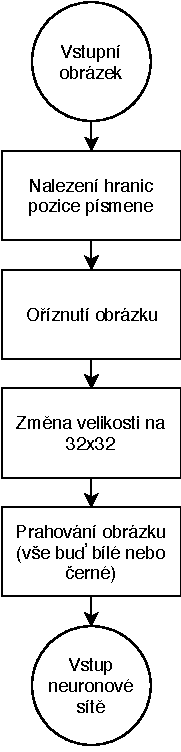
\includegraphics[]{FlowChartImageProcessing}
	\caption{Vývojový diagram znázorňující předzpracování obrázku, před klasifikací neuronovou sítí}
	\label{vyvojovy_diagram_zpracovani obrazku}
\end{figure}

Výsledkem této pomocné aplikace je soubor network.xml, s naučenou neuronovou sítí, který je poté použit (načten) v samotné aplikaci. Část funkcionality této aplikace je vytažena do dalšího samostatného projektu (knihovny) SmapCommon, tak aby aplikace, která bude písmena později dekódovat mohla využít stejného postupu, který byl využit pro zpracování obrázků, před předáním síti k učení (tj. funkce použité pro úpravy obrázků, budou používat stejně obě dvě aplikace, použitím knihovny se zajistí konzistence mezi oběma projekty).

Hlavní částí tohoto projektu je projekt smap, který implementuje samotné zakódovávání a dekódování dat. Jedná se o konzolovou aplikaci, která pracuje ve dvou režimech, kódování a dekódování. Pro zakódování dat na papír dle popisu z předchozí kapitoly, bylo zapotřebí najít a použít další vhodné knihovny, které by zajistili potřebnou funkcionalitu.

První z použitých knihoven je Cambia.BaseN, kterou aplikace využívá pro zakódování a dekódování dat do formátu Base64 a Base32. Tato knihovna je šířena pod open source licencí Microsoft Public License \cite{MicrosoftPublicLicense}, která jako v případě MIT licence, umožňuje využití v komerční sféře, aniž by nutila zveřejňovat zdrojové kódy, a nenutí odvození dílo šířit pod touto licencí.

Druhou použitou knihovnou je ZXing.Net. Jedná se o port Javovské knihovny ZXing, která je určená pro čtení a vytváření různých čárových kódu (EAN, Data matrix, QR kód,...). Jak již účel knihovny napovídá tuto knihovnu aplikace využívá k vytvoření QR kódu s meta daty při kódování dat a čtení QR kódu při dekódování dat. Tato knihovna je šířena pod open source licencí Apache 2.0 \cite{ApacheLicense}, opět jako v předchozím případě je možné ji používat v komerčních projektech a nenutí, aby aplikace, které využívají tuto knihovnu byly šířeny pod touto licencí.

Třetí použitou knihovnou je PDFsharp, kterou aplikace využívá pro vytvoření PDF souboru se zakódovanými data, tak aby je bylo snadné vytisknout. Tato knihovna je šířena pod MIT licencí jako SharpLearning, takže opět jsou zachovány stejné výhody jako v předchozím případě.

Poslední knihovnou, kterou aplikace využívá, která stojí za zmínku je SixLabors.ImageSharp. Jedná se o knihovnu sloužící pro manipulaci s 2D grafikou (obrázky), umožňující dělat různé pokročilejší operace s obrázky (ořezávání, rotace, změna měřítka,...). Tato knihovna je šířena pod licencí Apache 2.0, která nabízí stejné výhody jako v případě ZXing.Net.

Aplikace je implementována tak, že v případě kódování dat předpokládá na vstupu název souboru, který má zakódovat, výstupem je pak pdf soubor, který může být vytištěn. V případě dekódování aplikace na vstupu předpokládá adresář, který obsahuje obrázky (každý obrázek reprezentuje jednu naskenovanou stránku, aktuální implementace předpokládá, že stránky nejsou příliš mnoho natočeny, tj. QR kód by měl být vlevo nahoře, a stránky by měla být vychýlena pouze minimálně). Aplikace poté postupně provede několik kroků. Nejprve je zapotřebí dekódovat QR kód a to hned ze dvou důvodů. Prvním důvodem je získání metadat a druhým je, jak již bylo zmíněno v předchozí kapitole, detekce tzv. finder patters v QR kódu, na základě kterých se detekuje úhel vychýlení stránky, který vznikl například při automatickém podávání papírů do skeneru při skenováním do počítače. Pro dekódování QR kódů se používá již výše zmíněná knihovna ZXing.Net. 

Úhel vychýlení stránky se poté spočte tak, že se naleznou levé finder patterns v QR kódu, čímž získáme dva body v 2D prostoru. Pokud tyto dva body jsou rovnoběžné v ose Y, tak stránka s největší pravděpodobností není vychýlena/natočena. Pokud nejsou rovnoběžné jsme z těchto dvou bodů schopni spočítat délky odvěsen pravoúhlého trojúhelníku. Tyto strany lze poté využít k výpočtu úhlu vychýlení stránky pomocí goniometrické funkce tangens. To zda se jedná o natočení stránky po směru nebo proti směru hodinových ručiček se poté zjistí tak zda finder pattern umístěný na stránce výše je více nalevo (resp. napravo) než finder pattern umístěný níže.

% TODO listing ukázka spočtení úhlu tangens z finder patterns

Další věc, ke které se umístění QR kódu použije je k označení oblasti s písmeny na stránce. Jak již bylo řečeno předpokládá se, že stránka má QR kód umístěný vlevo nahoře, z tohoto důvodu není nutné řešit nutnost rotace celé stránky (v tomto případě je myšlena rotace o 90\degree, 180\degree nebo 270\degree). Za předpokladu, že platí umístění QR kódu vlevo nahoře, můžeme na základě finder patterns spočítat horní hranici stránky, kde začíná oblast s písmeny, kterou poté využijeme při dalším zpracování.

Před dalším zpracování je tedy stránka oříznuta a otočena, tak aby byla pokud možno rovně. Poté začíná samotné získávání jednotlivých písmen z obrazu. K tomuto účelu je použitý algoritmus podobný algoritmu scan line. Nejprve se snažíme získat jednotlivé řádky s textem, to se provede tak, že začneme úplně nahoře oříznutého obrázku a postupně kontrolujeme všechny horizontální pixely, pokud jsou bílé (barva pozadí, je zde opět využito metody prahování, tak aby se eliminoval šum, který by mohl vzniknout v důsledku skenování) tak se posouváme v ose Y. Jakmile narazíme na řádek (scan line), která obsahuje již černé pixely (tj. pixely s textem), tak si uložíme tuto souřadnici a pokračujeme v ,,skenování`` dalších řádků pixelů, ale s tím rozdílem, že hledáme první řádek, který bude celý složený z bílých pixelů. Jakmile jej najdeme, tak máme spočtenou horní a dolní souřadnici oblasti obsahující písmena řádku.

V rámci oblasti řádku poté pokračujeme naprosto stejně s tím rozdílem, že provádíme vertikální ,,skenování`` (tj. procházíme řádek v ose X). Tímto způsobem získáme oblasti jednotlivých písmen. Jakmile máme oblast písmene, můžeme s ním provést stejné kroky, které byly provedeny při učení neuronové sítě (tj. provedeme změnu měřítka, tak aby obrázek s písmenem byl veliký 32x32 pixelů a poté provedeme prahování). Při fázi dekódování provádíme prahování s dvěma různými parametry, tak abychom v případě, že nebude souhlasit kontrolní součet, mohli zkusit data dekódovat ještě jednou (aktuální řešení data porovnává pouze dvakrát, tj. vždy tak jak je klasifikuje neuronová síť, pro zvýšení stability by bylo vhodné v případě, že ani jedna sada znaků nesedí provést porovnání rozdílů obou sad znaků a vyzkoušet další rozdílné kombinace, pokud by se nějaké našli). 

Jak již bylo naznačeno po klasifikaci písmen je se použije neuronová sít, výstupem této klasifikace jsou číselné indexy, odpovídající pořadí písmene v kódovací abecedě. Díky tomu jsme schopni snadno tyto čísla převést na textový řetězec. Jakmile máme tento řetězec můžeme spočítat kontrolní součet pomocí hashovací funkce SHA1. Pokud se shoduje s kontrolním součtem uloženým v QR kódu, tak máme data dekódována správně (v tom případě si je připravíme do kolekce s uloženým indexem, určujícím jejich pořadí, a na pevný disk do složky s výstupem uložíme soubor obsahující tato dekódovaná data). V případě, že data jsou dekódována nekorektně je na standardní výstup aplikace vypsána informace o chybě a na pevný disk je uložen soubor, který je označen jako špatně dekódovaný, obsahující nesprávně klasifikovaná data (uživatel poté nemusí všechna data přepisovat do počítače ručně, ale provede pouze kontrolu, klasifikace dat v tomto souboru), tento případ užití by pokud možno neměl vůbec nastávat.

Výše zmíněné kroky se provedou pro všechny obrázky (stránky) ve vstupním adresáři. Nakonec pokud jsou všechny stránky dekódovány správně, se provede spojení textového obsahu stránek do jednoho textového řetězce, na základě pořadí čísel stránek. Tento textový řetězec je následně dekódován zpět na pole/sekvenci/blok bajtů. Tyto bajty jsou uloženy do výstupního souboru na pevný disk. Soubor by měl být naprosto identický s původním souborem, který byl na papír zakódován.

\section{Testing of developed application / Testování vyvinuté aplikace}

Po implementaci je nutné ověřit, zda vše funguje jak má. Z tohoto důvodu je nutné aplikaci otestovat. Jelikož se jedná o počítačový program, tak některé klíčové části aplikace (kódování a dekódování textových řetězců, parsování metadat) byly pokryty jednotkovými testy (unit testy). Na pokrytí veškeré funkcionality unit texty v rámci tohoto projektu bohužel nebyl čas. Z tohoto důvodu byla přidána sada ,,integračních`` testů, které zkoušejí tzv. end-to-end scénář (tj. provolávají existující aplikaci a zkoušejí, zda pro zadané vstupy vrací aplikace očekávaný výstup. Tj. výstupem testování aplikace je projekt Test, který obsahuje malou sadu unit testů a některé větší ,,integrační`` testy, které ověřují funkcionalitu celé aplikace. Tak aby se dalo prohlásit, že aplikace je napsaná ,,korektně`` a je funkční je zapotřebí aby všechny tyto testy procházely (tj. ,,byly zelené``).

Na začátku bylo pro účely testování vygenerováno několik souborů s náhodným obsahem, za pomoci speciálního linuxového soubor /dev/urandom, který slouží v linuxových systémech pro generování náhodných čísel (na operačním systému Windows lze tento soubor využít také, například pomocí GIT Bash, nebo Linux Subsystem for Windows (Linux Subsystem je dostupný pouze ve Windows 10)). Obsah dekódovaných souborů bude poté porovnáván vůči těmto souborům.

První sada ,,integračních`` testů testuje, strukturu/obsah vygenerovaných PDF souborů, jelikož PDF soubor obsahuje v sobě informaci o datu modifkace (takže i vytvoření), není možné binárně porovnat tzv. approve soubor (schválený soubor, tj. jedná se o soubor, který obsahuje očekávaná data, pokud výsledek běhu aplikace bude produkovat jiný soubor, pak někde nastala chyba a test by měl selhat) s nově vygenerovaným, protože by se neshodovaly minimálně v rámci těchto metadat. Z tohoto důvodu byly z vygenerovaných PDF souborů vytvořeny jpg soubory, která budou sloužit pro approve. Test tedy funguje tak, že máme v GITovém repositáři uloženy approve obrázky, které říkají, jak má výsledný výstup vypadat. Dále pak v testu provoláme zkompilovanou aplikaci, s argumenty, tak aby vygenerovala PDF soubor. Tento soubor poté převedeme na obrázek jpg a následně binárně porovnáme s approved obrázkem. Pokud v aplikaci není chyba, tak je vše bude v pořádku a test projde bez chyby, pokud se v aplikaci něco zásadního, co ovlivňuje výstup změní, tak test selže a dá vývojáři jasné znamení, že něco nemusí být v pořádku.

Druhá sada ,,integračních`` testů testuje, druhý mód programu, kterým je dekódování dat z obrázku. V těchto testech se nejprve připraví souborová struktura, kterou program potřebuje pro běh (tj. program očekává, že obrázkové soubory v nějakém adresáři reprezentují vždy jeden soubor. A také se připraví složka pro výstup programu). Následně je spuštěna zkompilovaná aplikace, s argumenty, které říkají co se má dekódovat. Poté co aplikace dokončí svůj běh, tak se zjistí, zda byl vygenerován soubor s jménem ,,encoded`` ve výstupním adresáři (tento soubor je výstupem dekódovacího procesu aplikace, pokud aplikace doběhla korektně, tak by měl existovat). Za předpokladu, že tento soubor existuje, tak je provedeno binární porovnání tohoto souboru s approved souborem. Pokud se soubory shodují tak test projde korektně. Pokud někde při dekódování nastala chyba, tak test neprojde a dává to vývojáři informaci o tom, že něco není v pořádku.

\subsection{Porovnání s jinými existujícími řešeními}

Jediné existující řešení, které vypadalo reálně použitelně je PaperBak. Porovnávat tato dvě řešení je relativně těžké, protože každý má trochu jiné priority při implementaci. Řešení implementované v rámci této práce mělo mít za cíl možnost snadného obnovení dat i v případě, že selže dekódovací program. Kdežto PaperBak je na straně druhé zaměřen na případ, kdy chceme uložit pokud možno co nejvíce dat na jeden papír. 

Jelikož řešení PaperBak využívá pro zapsání dat matice ,,čtverečků`` (tj. čárové kódy) umožňuje zapsat na jednu stranu A4 daleko více dat, nežli řešení implementované v rámci této práce. Na druhou stranu je, ale teoreticky daleko náročnější na kvalitu skenovacího a tiskového zařízení. Po vytištění stránky s řešením PaperBak člověka ani nenapadne, že by se pokoušel data dekódovat ručně, protože, již na první pohled je vidět, že by k dekódování bylo potřeba nezměrného úsilí a možná i mikroskopu. Na druhou stranu řešení implementované v rámci této práce by dekódovat ručně nemusel být příliš velký problém. Obě řešení jsou tedy použitelné, ale je zapotřebí zvážit jaké množství dat budeme zálohovat, a jak moc důvěřujeme programu, že je data schopen zpětně dekódovat. 

Pokud porovnáme rychlost dekódování dopadne řešení PaperBak výrazně lépe, protože nepotřebuje využívat relativně složitých výpočtů neuronových sítí na straně jedné a je daleko lépe optimalizované, nežli řešení implementované v rámci této práce (řešení implementované v rámci této práce slouží spíše jako prototyp/demonstrace možného řešení, tohoto problému, pokud by se mělo někde použít produkčně bylo by zapotřebí daleko více optimalizovat).

Výše popsané porovnání shrnuje následující tabulka \ref{tabulka:porovnani_reseni}.

\begin{table}[]
	\caption{Porovnání implementovaného řešení s řešením PaperBak \cite{PaperDataStorage}}
	\label{tabulka:porovnani_reseni}
	\begin{tabular}{|l|l|l|}
		\hline
		& PaperBak & Vlastní řešení \\ \hline
		Max. množství dat na 1 A4            & 488kB    & 1740B  \\ \hline
		Data zakódována v textu              & Ne       & Ano     \\ \hline
		Data zakódována do obrázku (kódu)    & Ano      & Ne      \\ \hline
		Možnost snadného dekódování člověkem & Ne       & Ano     \\ \hline
	\end{tabular}
\end{table}

\section{Conclusions / Závěry}

V rámci této práce jsme si daly za cíl vytvořit aplikaci, která bude schopna uložit počítačová data na papír a poté je zpátky načíst formou naskenovaného bitmapového obrázku. Jedním z hlavních cílů, kterých jsme se celou dobu držely bylo to, aby data byla čitelná i člověkem, z tohoto důvodu jsme zvolily datovou reprezentaci pomocí písmen. Pro určení/klasifikaci jednotlivých písmen jsme použili konvoluční neuronovou síť, kterou jsme musely naučit správně rozeznávat znaky fontu Consolas. V ideálních případech bylo dosaženo velice dobrých výsledků při klasifikaci znaků (Testy využívají soubory s daty jejichž velikost odpovídá 10,5kB pokud přepočteme na počet písmen dostaneme přibližně 16500 písmen, pokud zohledníme že se všechny tato písmena podařilo korektně dekódovat, získáme velice slušnou úspěšnost naučení neuronové sítě). 

V řešení vidím jistý potencionál. Pokud by se dotáhly různé neduhy tohoto řešení (malá hustota dat na jednu A4, rychlost dekódování, uživatelský komfort (konzolová aplikace se neobsluhuje příliš dobře),...) tak by se mohlo jednat o plnohodnotné řešení/alternativa k existujícímu řešení, pro zálohu dat na papír.

\begin{thebibliography}{1}

\bibitem{Ubicomp2001}
ABOWD,~Gregory D, Barry BRUMITT a Steven SHAFER. Ubicomp 2001: Ubiquitos Computing: International Conference Atlanta, Georgia, USA, September 30 - October 2, 2001 Proceedings. Springer-Verlag Berlin Heidelberg, 2001 [Cit. 16. Leden 2019]. ISBN: 978-3-540-45427-4. Dostupné z: https://doi.org/10.1007/3-540-45427-6

\bibitem{DataStorageLifespans}
MORGAN,~Casey. Data storage lifespans: How long will media really last?. 28. Srpen 2018 [Cit. 16. Leden 2019]. Dostupné z: https://blog.storagecraft.com/data-storage-lifespan/
	
\bibitem{ALSMADI2018218}
ALSMADI,~Duha a Victor PRYBUTOK. Sharing and storage behavior via cloud computing: Security and privacy in research and practice. 2018 [Cit. 16. Leden 2019]. ISSN: 0747-5632. Str. 218-226. Dostupné z: https://doi.org/10.1016/j.chb.2018.04.003

\bibitem{7MostFamousCloudSecurityBreaches}
BRADFORD,~Contel. 7 Most Infamous Cloud Security Breaches. 25. Červenec 2017 [Cit. 16. Leden 2019]. Dostupné z: https://blog.storagecraft.com/7-infamous-cloud-security-breaches/

\bibitem{HowSecureIsYourData}
ZHANG,~Haibin. How secure is your data when it’s stored in the cloud? 25. Leden 2018 [Cit. 16. Leden 2019]. Dostupné z: http://theconversation.com/how-secure-is-your-data-when-its-stored-in-the-cloud-90000

\bibitem{RecognizationVehicleLicencePlates}
CHANDRA,~S. 2017 20TH International Conference of Computer and Information Technology (ICCIT): An automated system to detect and recognize vehicle license plates of Bangladesh. 22.-24. Prosinec 2017 [Cit. 15. Leden 2019]. ISBN: 978-1-5386-1150-0. 
	
\bibitem{NIPS2010_4136}
NGIAM,~Jiquan a et al. Advances in Neural Information Processing Systems 23: Tiled convolutional neural networks. Curran Associates, Inc., 2010 [Cit. 14. Leden 2019]. str. 1279-1287. Dostupné z: http://papers.nips.cc/paper/4136-tiled-convolutional-neural-networks.pdf 

\bibitem{doi:10.1080/2150704X.2018.1526424}
ZHI,~Lu a et al. A dense convolutional neural network for hyperspectral image classification. Taylor \& Francis, 2019 [Cit. 15. Leden 2019]. str. 59-66. Dostupné z: https://doi.org/10.1080/2150704X.2018.1526424 

\bibitem{SEO2019328}
SEO,~Yian a Kyung-shik SHIN. Hierarchical convolutional neural networks for fashion image classification. 2019 [Cit. 15. Leden 2019]. str. 328-339. ISSN: 0957-4174. Dostupné z: https://doi.org/10.1016/j.eswa.2018.09.022

\bibitem{PaperDataStorage}
ATWOOD,~Jeff. The Paper Data Storage Option. 31. Července 2009 [Cit. 14. Leden 2019]. Dostupné z: https://blog.codinghorror.com/the-paper-data-storage-option/

\bibitem{GrantTrebbin}
TREBBIN,~Grant. Simple Data Backup with Paper Based QR Codes. 29. Květen 2015 [Cit. 14. Leden 2019]. Dostupné z: https://www.grant-trebbin.com/2015/05/encode-and-decode-file-backed-up-as.html  
	
\bibitem{DataGlyphsFreePatenstsOnline}
BREIDENBACH,~Jeff a David~L.~HECHT. Foreground/background document processing with dataglyphs: United States Patent 6641053. 4. Listopad 2003 [Cit. 14. Leden 2019]. Dostupné z: http://www.freepatentsonline.com/6641053.html

\bibitem{dataglyphs}
DataGlyphs®: Embedding Digital Data. [Cit. 14. Leden 2019]. Dostupné z: http://www.microglyphs.com/english/html/dataglyphs.shtml
	
\bibitem{PaperBackup}
paperbackup.py. 2017 [Cit. 14. Leden 2019]. Dostupné z: https://github.com/intra2net/paperbackup
  
\bibitem{PaperBak}
YUSCHUK,~Oleh. PaperBak. 2007 [Cit. 14. Leden 2019]. Dostupné z: http://ollydbg.de/Paperbak/

\bibitem{ScanningQrCodes}
SINHA,~Utkarsh. Scanning QR Codes: Introduction. [Cit. 14. Leden 2019] Dostupné z: http://www.aishack.in/tutorials/scanning-qr-codes-1/
  
\bibitem{Book:TheTypographicDeskReference}
ROSENDORF,~Theodore. The typographic desk reference: TDR. New Castle, DE: Oak Knoll Books, 2009. ISBN 978-1-58456-231-3.

\bibitem{RFC4648}
Josefsson,~S. The Base16, Base32, and Base64 Data Encodings. Říjen 2006 [Cit. 14. Leden 2019]. Dostupné z: https://tools.ietf.org/html/rfc4648

\bibitem{RFC3174}
EASTLAKE,~D.~3rd a JONES~P. US Secure Hash Algorithm 1 (SHA1). Září 2001 [Cit. 14. Leden 2019]. Dostupné z: https://tools.ietf.org/html/rfc3174

\bibitem{IEN137:LittleEndian}
COHEN,~Danny IEN 137: On Holy Wars and a Plea for Peace. 1. Duben 1980 [Cit. 14. Leden 2019]. Dostupné z: https://www.ietf.org/rfc/ien/ien137.txt

\bibitem{MITLicense}
WANG,~Kevin. MIT License (Expat) Explained in Plain English. 2015 [Cit. 14. Leden 2019]. Dostupné z: https://tldrlegal.com/license/mit-license

\bibitem{MicrosoftPublicLicense}
WANG,~Kevin. Microsoft Public License (MS-PL) Explained in Plain English. 2015 [Cit. 14. Leden 2019]. Dostupné z: https://tldrlegal.com/license/microsoft-public-license-(ms-pl)

\bibitem{ApacheLicense}
The~Apache~Software~Foundation. Apache License, Version 2.0. Leden 2004 [Cit. 14. Leden 2019]. Dostupné z: http://www.apache.org/licenses/LICENSE-2.0

\end{thebibliography}

\end{document}
